%; whizzy -pdf
\documentclass[12pt]{article}
\usepackage[pdftex]{graphicx}
\newcommand{\HRule}{\rule{\linewidth}{0.5mm}}
\usepackage{moreverb}
\usepackage{hyperref}
\usepackage{wrapfig}


\def\sourcetabsize{4}
\newenvironment{sourcestyle}{}{}%{\begin{scriptsize}}{\end{scriptsize}}
\def\sourceinput#1{\par\begin{sourcestyle}\verbatimtabinput[\sourcetabsize]{#1}\end{sourcestyle}\par}

\begin{document}
%\begin{titlepage}
\begin{center}

\includegraphics[width=1\textwidth]{./Hawk2.png}\\[0.5cm]
\HRule \\[0.4cm]
{\huge \bfseries Coding Standards}\\[0.1cm]
\HRule \\[1.0cm]
{\large Filipe R. N. C. Maia}\\[0.4cm]
{\large \today}\\[1.0cm]
\end{center}
%\end{titlepage}

%\title{{\huge \bfseries Hawk Coding Standards}}


%\author{Filipe R. N. C. Maia}
%\maketitle

\section{Introduction}
In the last few years Hawk has grown from a small program to a rather large one. Large programs bring
with it complexity and to try to fight this I decided to create a small set of rules for all the code
under Hawk and libspimage. These conventions should hopefully make the code more consistent and easier to read.

\section{General Rules}
\subsection{Floating point variables}
Throughout the program real should be used as the type for floating point variables.
This makes it easy to compile the program for either single or double precision. 
For variables which are seldom used, and as such negligible performance impact, for example those used in the graphical interface, float or double are acceptable.
\subsection{File location}
Source files should go under the /src directory. Documentation under /doc. 
Header files that are included from more than one location should go under /include. 
The rest of the header files should be in the same directory as the source files that includes it.

Resources such as images and stylesheets should go under the /src directory and placed close to where they are used.

\subsection{Header files}
All header files should start by checking if their filename is defined
and if not define it, and then conditionally define {\tt extern "C"},  as shown below:
\begin{sourcestyle}
\begin{verbatim}
#ifndef _LINEAR_ALG_H_
#define _LINEAR_ALG_H_ 1

... /* includes go here */

#ifdef __cplusplus
extern "C"
{
#endif /* __cplusplus */

... /* main code goes here */

#ifdef __cplusplus
}  /* extern "C" */
#endif /* __cplusplus */

#endif
\end{verbatim}
\end{sourcestyle}
This way we make sure never to include the same header file twice, and files can be included
from both C and C++.

\section{Rules for C based source code}
\subsection{C standard}
All code should be valid C99 as much as possible. Certain features of C99 should not yet 
be used such as complex numbers (unfortunately) as they are not widely supported.

\subsection{Variables, functions and structures}
All variables and functions should be all lowercase with words separated by underscores, 
for example:
\begin{sourcestyle}
\begin{verbatim}
int ignore_space_change_flag;
int remove_spaces(char * string_with_spaces);
\end{verbatim}
\end{sourcestyle}

Structures should use CamelCase and should be prefix in libspimage by Sp, e.g.:
\begin{sourcestyle}
\begin{verbatim}
typedef struct{
  SpPhasingConstraints constraints;
}SpPhasingERParameters;
\end{verbatim}
\end{sourcestyle}

\subsection{Macros enumerations and constants}
Macros should be all uppercase (e.g. {\tt M\_PI}). To define integer constants enumerations are preferred to macros, e.g.:
\begin{sourcestyle}
\begin{verbatim}
typedef enum{SpEnantiomorph=1,SpCorrectPhaseShift=2}SpSuperimposeFlags;
\end{verbatim}
\end{sourcestyle}
Enumerations names should use CamelCase as in the example. Constants for which enumerations are not suitable should use global const variables, e.g.:
\begin{sourcestyle}
\begin{verbatim}
const real EulerConstant = 2.718281828459045;
\end{verbatim}
\end{sourcestyle}
Global const variables should also use CamelCase.

\section{Rules for C++ based source code}
\subsection{File naming}
All C++ source files should have the ``.cpp'' extension. Files should only describe 
one class and the name of the file should be the same as the class name, except the file
name should be all lower case. For example the class {\tt ImageDisplay} is implemented in the file {\tt imagedisplay.cpp}. Header files should have the same name as the source file they define ({\tt imagedisplay.h } in this case).

\subsection{Classes and member variables and functions}
Classes should be named in CamelCase and there should be a simple mapping 
of one class per source file (e.g. {\tt ImageDisplay}, implemented in {\tt imagedisplay.cpp}).

Member functions should be in CamelCase with the first letter lower case (e.g {\tt ImageDisplay::initImageViewers()}).

All member variables should be private except in very special circumstances. 
The naming convention for member variables is the same as for member functions but with the ``m\_'' prefix in front (e.g. {\tt int m\_serverPort}).

For variables and member functions that begin with an acronym the entire acronym recomes lowercase (e.g. {\tt RPCServer * m\_rpcServer;})
\subsection{Macros enums and constants}
The rules for macros enumerations and constants are the same as for C, but with increased effort to avoid macros in C++.

\subsection{Forward declarations}
Forward declarations should be used in header files as much as possible to decrease coupling and compilation times.
For example use:
\begin{sourcestyle}
\begin{verbatim}
class B;

Class A{
 private:
  B * m_pointerToB;
}
\end{verbatim}
\end{sourcestyle}
instead of:
\begin{sourcestyle}
\begin{verbatim}
#include <b.h>

Class A{
 private:
  B * m_pointerToB;
}
\end{verbatim}
\end{sourcestyle}

\section{Rules related to the physical problem}


\subsection{Coordinate System}
\begin{wrapfigure}{r}{0.5\textwidth}
  \vspace{-40pt}
  \begin{center}
    \includegraphics[width=0.6\textwidth]{coordinate_diagram}
  \end{center}
  \vspace{-20pt}
  \caption{Pixels and positions on a 5x5 image.}
  \vspace{-10pt}
  \label{Fig:Coordinate}
\end{wrapfigure}

For 2D images Hawk defines the origin at the center of the top left pixel.
When talking about pixel number an image with size $width \times height$ will have
pixels ranging between $(0,0)$ to $(width-1,height-1)$. 

Since pixels have a finite size there's the need to address positions with
higher than pixel accuracy. We define these floating point positions to range
between $(-0.5,-0.5)$ at the top left corner of the $(0,0)$ pixel to
$(width-0.5,height-0.5)$ on the bottom right corner of the $(width-1,height-1)$
pixel.


\subsection{Use of Intensities and Amplitudes}
Throughout the program intensities should always be used for diffraction data
for which we do not know the phase (e.g. for the input data to {\tt
  uwrapc}). 

Amplitudes should exclusively be used for phased diffraction images,
in practice only calculated diffraction patterns.

\subsection{FFT Shifting}
Even though all FFT computations have to be performed with shifted data this
should be transparent to the user. The user should never see shifted images as
they are unnatural and unintuitive to most users and can be very confusing.

Shifted images should only be kept in memory in programs that have to do FFT
computations. All others programs should treat all images as if they were not shifted.

\end{document}